\documentclass[11pt,a4paper]{article}

% -----------------------------------------------------------------------------
% CS6868 Research Mini-Project Report Template
% -----------------------------------------------------------------------------
% Target length: 5-10 pages (including figures, excluding references).
% Compile with: latexmk -pdf main.tex
% -----------------------------------------------------------------------------

\usepackage[utf8]{inputenc}
\usepackage[T1]{fontenc}
\usepackage[margin=1in]{geometry}
\usepackage{microtype}
\usepackage{lmodern}
\usepackage{amsmath,amssymb}
\usepackage{graphicx}
\usepackage{booktabs}
\usepackage{array}
\usepackage{enumitem}
\usepackage{xcolor}
\usepackage{listings}
\usepackage{hyperref}
\usepackage[capitalise,noabbrev]{cleveref}
\usepackage{tikz}
\usetikzlibrary{shapes.multipart, positioning, arrows.meta}
\usepackage{pgfplots}
\pgfplotsset{compat=1.18}
\usepackage{subcaption}
\usepackage{placeins}

\hypersetup{
  colorlinks=true,
  linkcolor=black,
  citecolor=blue!60!black,
  urlcolor=blue!60!black,
}

% --- Listings style (for code snippets) ---------------------------------------
\definecolor{codegray}{gray}{0.95}
\definecolor{codegreen}{rgb}{0.0,0.5,0.0}
\definecolor{codepurple}{rgb}{0.5,0.0,0.35}
\lstset{
  basicstyle=\ttfamily\small,
  backgroundcolor=\color{codegray},
  frame=single,
  framesep=4pt,
  breaklines=true,
  columns=fullflexible,
  keepspaces=true,
  showstringspaces=false,
  keywordstyle=\color{codepurple}\bfseries,
  commentstyle=\color{codegreen},
  stringstyle=\color{blue!60!black},
}

% --- Title block --------------------------------------------------------------
\title{%
  \textbf{CS6868 Research Mini-Project} \\[0.3em]
  \Large Concurrent Hash Maps: Striped Locking vs.\ Split-Ordered Lists%
}
\author{%
  Ogirala Srihasa \\ \texttt{cs25m034@smail.iitm.ac.in}
  \and
  Botla Venkata Ramamohan Rao \\ \texttt{cs25m017@smail.iitm.ac.in}
}
\date{\today}

\begin{document}
\maketitle

\begin{abstract}
Concurrent hash maps are a foundational data structure in multicore software, requiring careful trade-offs between implementation complexity, contention overhead, and scalability. We implement and comparatively evaluate two designs in OCaml 5: a \emph{striped-locking} hash map, which partitions buckets across mutex-protected stripes with stop-the-world resizing, and a \emph{lock-free split-ordered list }hash map, which encodes all entries in a single CAS-based linked list sorted by bit-reversed hash keys, enabling incremental resizing without rehashing. Both implementations are realised as functors over arbitrary key types and verified for correctness using QCheck-Lin, QCheck-STM (sequential consistency), and Thread Sanitizer (data-race detection), which together uncovered and guided the resolution of bugs during development. Benchmarks across 1–8 threads and three workload profiles — read-heavy, write-heavy, and mixed — show that the split-ordered design achieves up to 4.2× higher throughput under read-heavy workloads at 8 threads and maintains 3.5× higher throughput during active resizing, at the cost of 1.7× higher memory overhead. These results confirm that lock-free designs offer meaningful scalability advantages in OCaml 5's multicore runtime.
\end{abstract}

% =============================================================================
\section{Goals}
\label{sec:goals}
% =============================================================================

Hash maps are among the most widely used data structures in systems
programming, and making them thread-safe without sacrificing throughput is a
central challenge in concurrent programming. This project implements and
compares two fundamentally different approaches to concurrent hashing in
OCaml~5:
\begin{enumerate}[leftmargin=*]
  \item \textbf{Striped locking} — the bucket array is partitioned into
    mutex-protected stripes, enabling coarse-grained parallelism. This design
    extends the striped hash set presented in Chapter~13 of
    \emph{The Art of Multiprocessor Programming}~\cite{AoMPP} to a full
    key-value hash map, using standard \texttt{Mutex} primitives for
    stripe-level locking with dynamic resizing.
  \item \textbf{Split-ordered lists} — a lock-free design introduced by
    Shalev and Shavit~\cite{ShalevShavit2006} and discussed in Chapter~13
    of \emph{The Art of Multiprocessor Programming}~\cite{AoMPP}. We extend
    the original hash set formulation to support arbitrary key-value
    mappings, enabling lock-free resizing without rehashing.
\end{enumerate}
Both implementations support \texttt{insert}, \texttt{find}, \texttt{remove},
and \texttt{size}, with dynamic resizing under load.
\medskip
\noindent

\textbf{Research question.} \emph{Does the lock-free split-ordered
list design provide meaningful throughput advantages over striped locking under
read-heavy workloads, and how do the two approaches compare during concurrent
resizing?}

% =============================================================================
\section{Background}
\label{sec:background}
% =============================================================================
\subsection{Striped locking}

A striped hash map maintains an array of \emph{buckets}, where each bucket is
a list of key-value pairs sharing the same hash modulo the bucket count.
To enable concurrency without a single global lock, the array is partitioned
into $N$ \emph{stripes}, where bucket~$i$ is guarded by stripe $i \bmod
N$~\cite{AoMPP}. Operations on different stripes proceed in parallel; those on
the same stripe serialise. Each operation computes the target bucket, acquires
the corresponding stripe lock, and scans the bucket's list for the key.

As nodes accumulate, bucket lists grow and lookup degrades from $O(1)$ toward
$O(n)$. When the load factor --- stored entries divided by bucket count ---
exceeds~$0.75$, the map \emph{resizes}: all $N$ stripe locks are acquired in
ascending index order (to prevent deadlock), the bucket array is doubled, every
entry is rehashed into its new position, and the locks are released. No other
thread may access the map during this window, making resize a
\emph{stop-the-world} event and the primary scalability bottleneck of the
striped design.


\subsection{Split-ordered lists}
A split-ordered hash map stores all nodes in a \emph{single} lock-free linked
list sorted by a \emph{split-ordered key}: the bit-reversal of the node's hash,
with the LSB forced to~1 for data nodes and to~0 for sentinel nodes. The LSB
convention ensures every sentinel sorts strictly before the data nodes of its
bucket. Ties in split-ordered key (caused by hash collisions) are broken by
\texttt{K.compare} on the original keys.

To avoid scanning from the list head, the map maintains an array of
\emph{sentinel} pointers as indexed entry points at bucket boundaries. An
operation on bucket~$b$ begins traversal from $b$'s sentinel, bounding the
scan to that bucket's nodes alone. All insertions and removals use
compare-and-set (\textsc{cas}) on node next-pointers, following the
Harris two-phase protocol from Lecture~7.

Resizing is \emph{incremental}: when the load factor exceeds~$2.0$, the
logical bucket count is doubled from $B$ to $2B$ with a single \textsc{cas} on
an atomic counter. No node moves. Because bit-reversal maps higher hash bits to
lower sort-key positions, the nodes of bucket~$b$ already partition in sorted
order into those that remain in~$b$ and those that migrate to~$b+B$ — the
split requires no relinking.

Sentinel nodes are created \emph{lazily} on first access. The sentinel for
bucket~$b$ is inserted starting from the sentinel of $b$'s \emph{parent} —
the bucket obtained by stripping the highest set bit of~$b$ (e.g.\
$\text{parent}(5) = \text{parent}(101_2) = 001_2 = 1$) — which is always the
closest preceding entry point in the sorted list. If the parent sentinel does
not yet exist it is initialised recursively; the recursion terminates at
bucket~0, whose sentinel is the permanent list head. Because resize acquires no
locks and touches no existing nodes, all threads continue operating throughout
— making resize fully concurrent and the primary scalability advantage over
striped locking.
% =============================================================================
\section{Tasks Undertaken}
\label{sec:tasks}

\subsection{Implementation}

The complete implementation can be found at the public \href{https://github.com/ogirala-srihasa/Concurrent-Hashmap/tree/main}{github repo}

Both hash maps are realised as OCaml functors parameterised over a \texttt{KEY}
module (defined in \href{https://github.com/ogirala-srihasa/Concurrent-Hashmap/blob/main/lib/hashmap_intf.ml}{\texttt{hashmap\_intf.ml}}), which must supply a type \texttt{t},
a \texttt{hash} function, an \texttt{equal} predicate, and a \texttt{compare}
function. Both functors produce a module satisfying the \texttt{HASHMAP}
signature, exposing \texttt{create}, \texttt{insert}, \texttt{find},
\texttt{remove}, and \texttt{size}. This common interface allows the benchmark
and test harnesses to swap one implementation for the other with a single
module alias change. For the lock free implementation we used the \texttt{AtomicMarkableRef} from lecture 7



% -----------------------------------------------------------------------------
\subsubsection{Striped locking hash map (\href{https://github.com/ogirala-srihasa/Concurrent-Hashmap/blob/main/lib/striped_hashmap.ml}{\texttt{striped\_hashmap.ml}})}
% -----------------------------------------------------------------------------

\paragraph{Data structure.}
The striped hash map stores nodes in a bucket array, where each bucket is an
OCaml association list of \texttt{(key, value)} pairs sharing the same hash
modulo the bucket count (separate chaining). The record type is:

\begin{verbatim}
type 'v t = {
  buckets  : (K.t * 'v) list array Atomic.t;
  locks    : Mutex.t array;
  num_stripes      : int;
  size     : int Atomic.t;
  capacity : int Atomic.t;
  load_factor_threshold : float;
  resize_lock : Mutex.t;
}
\end{verbatim}

Both \texttt{buckets} and \texttt{capacity} are wrapped in \texttt{Atomic.t}.
This was a deliberate design decision made after ThreadSanitizer (Section
\ref{sec:tsan}) reported data races on both fields: \texttt{capacity} was read
by \texttt{should\_resize} without any lock held, and the \texttt{buckets}
pointer was swapped by \texttt{resize} while readers held only one stripe lock.
Making both fields atomic eliminates the races without requiring callers to hold
any additional locks.

\paragraph{Stripe assignment.}
Bucket $i$ is guarded by stripe $i \bmod N$, where $N$ is the configurable
stripe count (default 16). A \texttt{Mutex.t array} of length $N$ is allocated
at creation and never changes. The number of stripes is kept less than or equal
to the initial capacity to ensure every stripe guards at least one bucket.

\paragraph{Operations.}
Each of \texttt{insert}, \texttt{find}, and \texttt{remove} follows the same
retry protocol:
\begin{enumerate}
  \item Compute the bucket index $b$ and stripe index $s = b \bmod N$.
  \item Acquire \texttt{locks.(s)}.
  \item Recompute the bucket index $b'$ under the lock.
  \item If $b \neq b'$, a concurrent resize changed \texttt{capacity} between
        steps~1 and~2, moving the key to a different stripe. Release the lock
        and restart from step~1.
  \item Otherwise, operate on the chain at \texttt{buckets.(b)} and release.
\end{enumerate}

The re-validation in step~4 is a subtle but essential correctness condition.
Without it, a thread that computed its bucket index before a resize could
write to the wrong bucket after the resize doubled the array.

\texttt{insert} performs an upsert: if the key already exists in the chain, it
rebuilds the chain with the new value using \texttt{List.map} rather than
removing and re-inserting, avoiding a window in which the key is temporarily
absent. If the key is new, it is prepended to the chain and \texttt{size} is
incremented atomically.

\paragraph{Dynamic resizing.}
After every \texttt{insert}, \texttt{should\_resize} checks whether the load
factor $\lvert\text{size}\rvert / \lvert\text{capacity}\rvert$ exceeds the
threshold (default 0.75). If so, \texttt{resize} is called outside the stripe
lock. \texttt{resize} first acquires a dedicated \texttt{resize\_lock} (so only
one resize runs at a time), double-checks the condition, then acquires all $N$
stripe locks in strictly ascending index order. Ascending order prevents
deadlock: any two threads that attempt to acquire the same set of locks will
always request them in the same order. With all stripes held, the bucket array
is doubled, every entry is rehashed into the new array, and \texttt{buckets}
and \texttt{capacity} are updated atomically via \texttt{Atomic.set} before
releasing the locks. This is a stop-the-world event: no other thread may
read or write the map during the resize window.

% -----------------------------------------------------------------------------
\subsubsection{Split-ordered list hash map (\href{https://github.com/ogirala-srihasa/Concurrent-Hashmap/blob/main/lib/split_ordered_hashmap.ml}{\texttt{split\_ordered\_hashmap.ml}})}
% -----------------------------------------------------------------------------

\paragraph{Data structure.}
The split-ordered map stores all nodes in a single lock-free linked list sorted
by a \emph{split-ordered key}. Each node in the list has the following type:

\begin{verbatim}
type 'v node = {
  so_key   : int;
  real_key : K.t;
  value    : 'v option Atomic.t;
  next     : 'v node AMR.t;
}
\end{verbatim}

\texttt{so\_key} is the bit-reversed sort key that determines the node's
position in the global list. \texttt{real\_key} is the original unhashed key,
used as a tiebreaker when two nodes share the same \texttt{so\_key} due to a
hash collision. \texttt{value} is wrapped in \texttt{Atomic.t} to allow
in-place value updates without removing and re-inserting the node, eliminating
any window in which the key would be temporarily absent. \texttt{next} is an
\texttt{AtomicMarkableRef} rather than a plain pointer, pairing the next-node
reference with a boolean mark bit; setting the mark bit to \texttt{true}
signifies that this node is logically deleted and should be physically unlinked
during the next traversal of that region of the list. Sentinel nodes use the
same type but carry a placeholder \texttt{sentinel\_dummy\_key} (an
\texttt{Obj.magic 0} value) in \texttt{real\_key} and \texttt{None} in
\texttt{value}; the \texttt{node\_less\_than} and \texttt{node\_equal\_key}
helpers guard against passing this placeholder to \texttt{K.compare} by only
invoking it when both nodes are regular (LSB = 1 in \texttt{so\_key}).

The table itself is represented by the following record:

\begin{verbatim}
type 'v t = {
  head         : 'v node;
  buckets      : 'v node option Atomic.t array;
  bucket_count : int Atomic.t;
  max_buckets  : int;
  size         : int Atomic.t;
  load_factor_threshold : float;
}
\end{verbatim}

\texttt{max\_buckets} is a fixed physical upper bound allocated at creation
(default: initial capacity $\times$ 256, permitting up to eight doublings).
\texttt{bucket\_count} is the logical active size and grows via CAS during
resize. \texttt{buckets} is a pre-allocated sentinel pointer array; slots
beyond \texttt{bucket\_count} are uninitialised (\texttt{None}) until lazily
populated.

\paragraph{Key encoding and bit reversal.}
Two functions encode keys as sort keys for the global list:

\begin{verbatim}
let make_regular_key h  = (reverse_bits h) lor 1
let make_sentinel_key i = (reverse_bits i) land (lnot 1)
\end{verbatim}

\texttt{reverse\_bits} reverses all 62 non-sign bits of an OCaml integer (63
bits on 64-bit systems, minus the sign bit). Forcing the LSB to~1 for regular
nodes and to~0 for sentinel nodes ensures every sentinel sorts strictly before
the data nodes of its own bucket, since they share the same upper bits but
differ in the LSB position ($0 < 1$).

The raw hash is masked to \texttt{max\_int - 1} before bit reversal, ensuring
the result never equals \texttt{max\_int}, which is reserved for the tail
sentinel's sort key.

\paragraph{Collision handling.}
Because \texttt{hash\_key} can map two distinct keys to the same integer, two
regular nodes may share the same split-ordered key. To prevent silent key
loss or incorrect value returns, all list operations use a \emph{composite}
sort key \texttt{(so\_key, real\_key)}: nodes with equal \texttt{so\_key} are
further ordered by \texttt{K.compare} on their original keys. The helpers
\texttt{node\_less\_than} and \texttt{node\_equal\_key} only invoke
\texttt{K.compare} when both nodes are regular (LSB = 1), so the
\texttt{sentinel\_dummy\_key} placeholder (an \texttt{Obj.magic 0} value used
for sentinel and tail nodes) is never passed to \texttt{K.compare}.

\paragraph{Lock-free list operations.}
\texttt{locate} finds the \texttt{(pred, curr)} window around a target key,
physically snipping out logically deleted nodes along the way via CAS. If a
snip CAS fails (a concurrent thread already snipped the node), \texttt{locate}
restarts from the sentinel rather than the list head, bounding the retry scope.

Removal uses the Harris two-phase protocol: \texttt{list\_remove}
first marks \texttt{curr.next} atomically (logical deletion), then attempts a
best-effort CAS to physically unlink \texttt{curr} from \texttt{pred.next}.
Physical unlinking is best-effort because subsequent \texttt{locate} calls will
snip any remaining marked nodes during their traversal. The logical mark is
critical: without it, a concurrent \texttt{list\_insert} immediately after
\texttt{curr} could be silently lost when the physical-unlink CAS discards the
freshly inserted node.

\texttt{insert} performs an atomic in-place value update when a key already
exists: rather than removing and re-inserting (which would create a window
where the key is absent), it locates the existing node and calls
\texttt{Atomic.set} on its \texttt{value} field directly.

\paragraph{Lazy sentinel initialisation.}
\texttt{get\_bucket t idx} returns the sentinel node for bucket \texttt{idx},
calling \texttt{init\_bucket t idx} if the slot is \texttt{None}.
\texttt{init\_bucket} inserts the new sentinel starting from the
\emph{parent} bucket's sentinel rather than the list head. The parent of
bucket $b$ is obtained by stripping the highest set bit of $b$:
for example, $\text{parent}(5) = \text{parent}(101_2) = 001_2 = 1$.
This relationship reflects the doubling structure of resize: bucket $b$ is
created by splitting its parent, so the parent sentinel is always the
closest preceding entry point in the sorted list. If the parent sentinel
does not yet exist, \texttt{init\_bucket} initialises it recursively first;
the recursion always terminates at bucket 0, whose sentinel is the permanent
list head. Because multiple threads may race to initialise the same sentinel,
\texttt{init\_bucket} always calls \texttt{list\_find} after the insert attempt
to read back whichever sentinel won the race, and stores that pointer into the
\texttt{buckets} array.

\paragraph{Incremental lock-free resizing.}
\texttt{maybe\_resize} doubles \texttt{bucket\_count} with a single CAS if the
load factor exceeds the threshold (default 2.0, higher than striped because
per-bucket traversal cost is lower). No node moves, no lock is acquired, and
no thread is blocked. When the bucket count doubles from $B$ to $2B$, the
nodes in bucket $b$ naturally split into those that remain in bucket $b$ and
those that now belong to bucket $b + B$, as determined by the next bit of
their bit-reversed hash. This split is already encoded in the existing sort
order of the list and requires no relinking.

% =============================================================================
\subsection{Testing and Verification}
\label{sec:testing}
% =============================================================================

We applied three complementary verification techniques to both implementations:
manual unit tests, property-based concurrency tests (QCheck-Lin and QCheck-STM),
and ThreadSanitizer. Together they uncovered and guided the resolution of
bugs during development.

% -----------------------------------------------------------------------------
\subsubsection{Manual unit tests}

Both \href{https://github.com/ogirala-srihasa/Concurrent-Hashmap/blob/main/test/test_striped.ml}{\texttt{test\_striped.ml}} and \href{https://github.com/ogirala-srihasa/Concurrent-Hashmap/blob/main/test/test_split_ordered.ml}{\texttt{test\_split\_ordered.ml}} have implementation of the following tests: sequential operations, error handling,
concurrent inserts, concurrent mixed operations, resize correctness,
no-lost-items (striped only), concurrent resize stress (split-ordered only),
negative integer keys, string keys, and float keys.

% -----------------------------------------------------------------------------
\subsubsection{QCheck-STM}
% -----------------------------------------------------------------------------

\href{https://github.com/ogirala-srihasa/Concurrent-Hashmap/blob/main/test/qcheck_stm_striped.ml}{\texttt{qcheck\_stm\_striped.ml}} and \href{https://github.com/ogirala-srihasa/Concurrent-Hashmap/blob/main/test/qcheck_stm_split_ordered.ml}{\texttt{qcheck\_stm\_split\_ordered.ml}}
use QCheck-STM to test both implementations against a sequential reference
model. The model is OCaml's \texttt{Hashtbl} with functional semantics: the
state is an association list of \texttt{(key, value)} pairs, and each command
(\texttt{Insert}, \texttt{Find}, \texttt{Remove}, \texttt{Size}) has a
corresponding \texttt{next\_state} transformer and \texttt{postcond} check.

% -----------------------------------------------------------------------------
\subsubsection{QCheck-Lin}
% -----------------------------------------------------------------------------

\href{https://github.com/ogirala-srihasa/Concurrent-Hashmap/blob/main/test/qcheck_lin_striped.ml}{\texttt{qcheck\_lin\_striped.ml}} and \href{https://github.com/ogirala-srihasa/Concurrent-Hashmap/blob/main/test/qcheck_lin_split_ordered.ml}{\texttt{qcheck\_lin\_split\_ordered.ml}} each test generates 1\,000 random
concurrent \texttt{insert}/\texttt{find}/\texttt{remove} sequences across two
domains and checks that some valid sequential interleaving of the observed
results exists, again using \texttt{Hashtbl} as the reference model.

The \texttt{size} operation is deliberately excluded from the Lin tests for
both implementations. In both designs, the \texttt{size} counter
(\texttt{int Atomic.t}) is incremented or decremented \emph{after} the
structural change (insert or remove) has been committed. There is therefore
a brief window in which the structure has changed but \texttt{size} has not
yet been updated, making \texttt{size} inherently non-linearizable with
respect to the structural operations. This is an accepted and documented
limitation of the counter design.

% -----------------------------------------------------------------------------
\subsubsection{ThreadSanitizer (TSAN)}
\label{sec:tsan}
% -----------------------------------------------------------------------------

Both implementations were run under ThreadSanitizer using OCaml~5's dedicated
\texttt{5.4.0+tsan} opam switch, which instruments the runtime for data-race
detection. The manual concurrent tests (\href{https://github.com/ogirala-srihasa/Concurrent-Hashmap/blob/main/test/test_striped.ml}{\texttt{test\_striped.ml}},
\href{https://github.com/ogirala-srihasa/Concurrent-Hashmap/blob/main/test/test_split_ordered.ml}{\texttt{test\_split\_ordered.ml}}) were used as the TSAN workloads since they
exercise the highest level of concurrency.

TSAN reported two distinct data races on the striped implementation and no
races on the split-ordered implementation.

\paragraph{Race 1 — \texttt{should\_resize} reads \texttt{capacity} with no lock.}
\texttt{should\_resize} was called before acquiring any stripe lock, and read
\texttt{t.capacity} as a plain \texttt{int} while \texttt{resize} was writing
it under all stripe locks. TSAN identified the conflict as a write in
\texttt{camlStriped\_hashmap.fun\_697} (the resize closure) racing with a
read in \texttt{camlStriped\_hashmap.should\_resize\_394}.

\paragraph{Race 2 — \texttt{bucket\_for\_key} reads \texttt{capacity} before
acquiring the stripe lock.}
In the \texttt{attempt} loop, \texttt{bucket\_for\_key} is called \emph{first}
to compute the initial bucket index, and only then is the corresponding stripe
lock acquired. This first call reads \texttt{t.capacity} with \emph{no} stripe
lock held. Concurrently, \texttt{resize} writes \texttt{t.capacity} while
holding all $N$ stripe locks. The read and write are therefore wholly
unsynchronised.

\paragraph{Fix.}
Both fields \texttt{capacity} and \texttt{buckets} were changed from plain
mutable record fields to \texttt{int Atomic.t} and
\texttt{(K.t * 'v) list array Atomic.t} respectively. All reads were updated
to \texttt{Atomic.get} and all writes to \texttt{Atomic.set}. After this
change, TSAN reported no races on either implementation.

% -----------------------------------------------------------------------------
\subsubsection{Bugs discovered}
% -----------------------------------------------------------------------------

The three verification layers together uncovered bugs during development:

\begin{enumerate}

  \item \textbf{Sentinel key collision with tail} (split-ordered) — using
        \texttt{land max\_int} instead of \texttt{land (max\_int - 1)} in
        \texttt{hash\_key} allowed the tail sentinel's sort key (\texttt{max\_int})
        to be produced by a real key, breaking list termination. Caught by
        the manual boundary-key tests.
        
  \item \textbf{Wrong bucket after resize in striped} — the retry loop in
        \texttt{insert}/\texttt{find}/\texttt{remove} did not re-validate the
        bucket index after acquiring the stripe lock. A concurrent resize
        between the index computation and the lock acquisition could place
        the operation in the wrong bucket. Caught by the STM concurrent tests
        and fixed by re-computing and comparing the bucket index inside the lock.

  \item \textbf{Data race on \texttt{capacity} and \texttt{buckets}} (striped)
        — as described in Section~\ref{sec:tsan}, both fields were unprotected
        plain record fields. Caught by TSAN and fixed by making both
        \texttt{Atomic.t}.
\end{enumerate}
% =============================================================================
\section{Evaluation}
\label{sec:evaluation}

\subsection{Experimental setup}

All benchmarks were run on an Apple MacBook Air M4 (8 performance cores,
16\,GB RAM) under OCaml~5 with the default runtime. Thread counts ranged from
1 to 8. Each configuration was repeated 10 times and averaged. Three workload
profiles were tested: read-heavy (90/5/5 find/insert/remove), write-heavy
(10/45/45), and mixed (50/25/25), each with 500{,}000 operations per thread
and 1{,}000 pre-populated entries. A separate resize benchmark used an 80\%
insert workload starting from capacity~4 to stress concurrent resizing.

% ---------------------------------------------------------------------------
\subsection{Throughput scaling}
% ---------------------------------------------------------------------------

\Cref{fig:throughput-read,fig:throughput-write,fig:throughput-mixed} plots
throughput in millions of operations per second as thread count increases
across all three workload profiles.

\begin{figure}[ht]
\centering
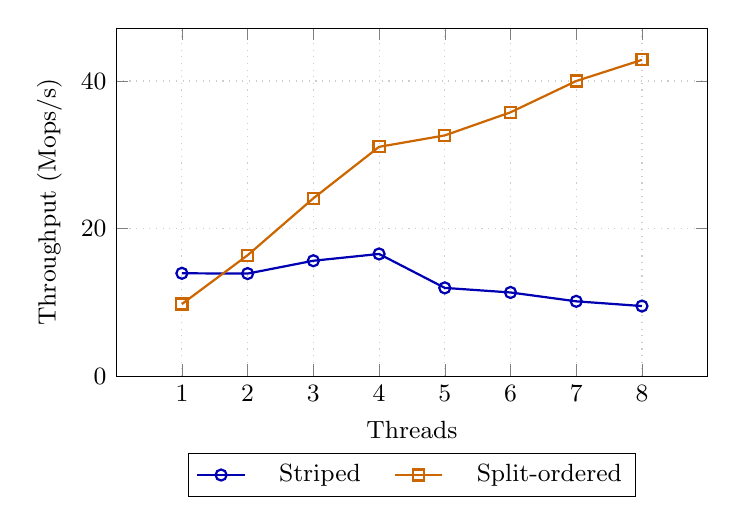
\begin{tikzpicture}
\begin{axis}[
  width=0.75\linewidth, height=6cm,
  xlabel={Threads}, ylabel={Throughput (Mops/s)},
  xtick={1,2,3,4,5,6,7,8},
  xmin=0, xmax=9, ymin=0,
  grid=major, grid style={dotted,gray!40},
  legend style={font=\small, at={(0.5,-0.22)}, anchor=north,
                legend columns=2, column sep=1em},
  tick label style={font=\small},
  label style={font=\small},
]
\addplot[color=blue!70!black, mark=o, thick] coordinates {
  (1,13.94)(2,13.90)(3,15.64)(4,16.56)(5,11.96)(6,11.34)(7,10.14)(8,9.50)};
\addplot[color=orange!80!black, mark=square, thick] coordinates {
  (1,9.77)(2,16.39)(3,24.10)(4,31.08)(5,32.63)(6,35.76)(7,40.00)(8,42.87)};
\legend{Striped, Split-ordered}
\end{axis}
\end{tikzpicture}
\caption{Throughput (Mops/s) vs.\ thread count --- read-heavy workload
(90/5/5 find/insert/remove, 500K ops/thread, average of 10 runs).}
\label{fig:throughput-read}
\end{figure}

\begin{figure}[ht]
\centering
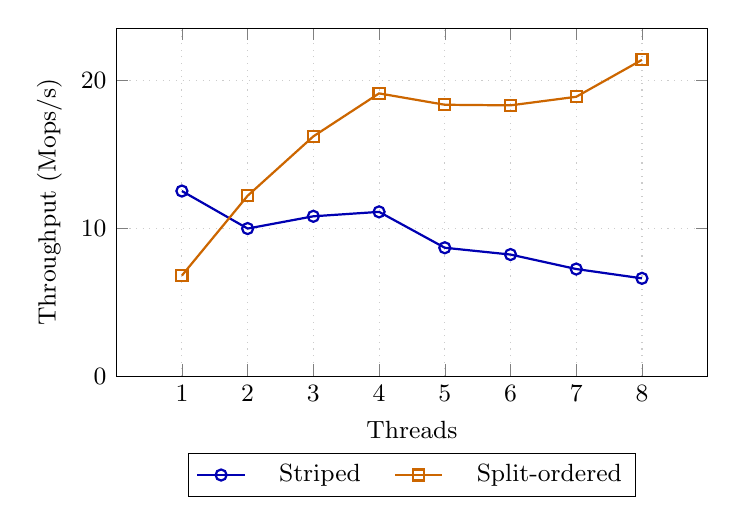
\begin{tikzpicture}
\begin{axis}[
  width=0.75\linewidth, height=6cm,
  xlabel={Threads}, ylabel={Throughput (Mops/s)},
  xtick={1,2,3,4,5,6,7,8},
  xmin=0, xmax=9, ymin=0,
  grid=major, grid style={dotted,gray!40},
  legend style={font=\small, at={(0.5,-0.22)}, anchor=north,
                legend columns=2, column sep=1em},
  tick label style={font=\small},
  label style={font=\small},
]
\addplot[color=blue!70!black, mark=o, thick] coordinates {
  (1,12.53)(2,9.99)(3,10.82)(4,11.12)(5,8.69)(6,8.23)(7,7.25)(8,6.62)};
\addplot[color=orange!80!black, mark=square, thick] coordinates {
  (1,6.81)(2,12.21)(3,16.23)(4,19.14)(5,18.37)(6,18.33)(7,18.91)(8,21.41)};
\legend{Striped, Split-ordered}
\end{axis}
\end{tikzpicture}
\caption{Throughput (Mops/s) vs.\ thread count --- write-heavy workload
(10/45/45 find/insert/remove, 500K ops/thread, average of 10 runs).}
\label{fig:throughput-write}
\end{figure}

\begin{figure}[ht]
\centering
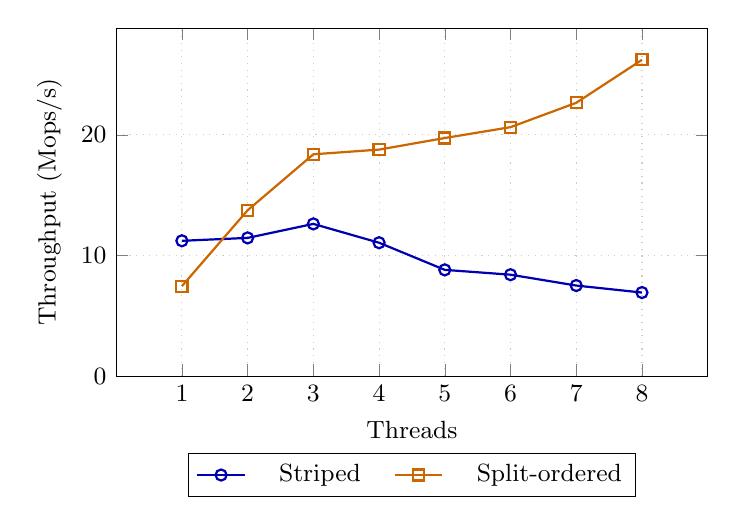
\begin{tikzpicture}
\begin{axis}[
  width=0.75\linewidth, height=6cm,
  xlabel={Threads}, ylabel={Throughput (Mops/s)},
  xtick={1,2,3,4,5,6,7,8},
  xmin=0, xmax=9, ymin=0,
  grid=major, grid style={dotted,gray!40},
  legend style={font=\small, at={(0.5,-0.22)}, anchor=north,
                legend columns=2, column sep=1em},
  tick label style={font=\small},
  label style={font=\small},
]
\addplot[color=blue!70!black, mark=o, thick] coordinates {
  (1,11.22)(2,11.46)(3,12.62)(4,11.06)(5,8.81)(6,8.41)(7,7.51)(8,6.93)};
\addplot[color=orange!80!black, mark=square, thick] coordinates {
  (1,7.46)(2,13.75)(3,18.39)(4,18.78)(5,19.74)(6,20.64)(7,22.66)(8,26.22)};
\legend{Striped, Split-ordered}
\end{axis}
\end{tikzpicture}
\caption{Throughput (Mops/s) vs.\ thread count --- mixed workload
(50/25/25 find/insert/remove, 500K ops/thread, average of 10 runs).}
\label{fig:throughput-mixed}
\end{figure}

\paragraph{Observations.}
At 1 thread, the striped map is faster across all workloads due to its lower
per-operation cost: bucket-chain reads require no CAS and no atomic pointer
traversal. However, stripe-lock contention causes striped throughput to
degrade beyond 4 threads, settling at 6--10\,Mops/s by 8 threads regardless
of workload.

The split-ordered list scales near-linearly through all 8 performance cores,
peaking at 42.9\,Mops/s under the read-heavy workload at 8 threads ---
$4.5\times$ the striped map. Under write-heavy load the advantage is reduced
($3.2\times$ at 8 threads) because failed CAS retries on the linked list are
more expensive than a simple list mutation under a stripe lock. Nevertheless,
the lock-free design retains positive scaling through 8 threads across all
workloads, whereas the striped map degrades monotonically beyond 4 threads.

% ---------------------------------------------------------------------------
\subsection{Resize benchmark}
% ---------------------------------------------------------------------------

\begin{figure}[ht]
\centering
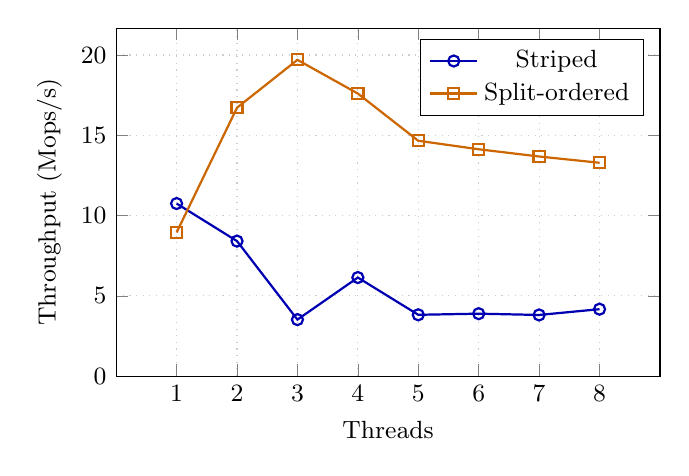
\begin{tikzpicture}
\begin{axis}[
  width=0.70\linewidth, height=6cm,
  xlabel={Threads}, ylabel={Throughput (Mops/s)},
  xtick={1,2,3,4,5,6,7,8},
  xmin=0, xmax=9, ymin=0,
  grid=major, grid style={dotted,gray!40},
  legend style={font=\small, at={(0.97,0.97)}, anchor=north east},
  tick label style={font=\small},
  label style={font=\small},
]
\addplot[color=blue!70!black, mark=o, thick] coordinates {
  (1,10.75)(2,8.41)(3,3.52)(4,6.14)(5,3.82)(6,3.89)(7,3.81)(8,4.17)};
\addplot[color=orange!80!black, mark=square, thick] coordinates {
  (1,8.95)(2,16.72)(3,19.70)(4,17.60)(5,14.66)(6,14.13)(7,13.68)(8,13.29)};
\legend{Striped, Split-ordered}
\end{axis}
\end{tikzpicture}
\caption{Throughput during active resizing (80\% inserts, initial capacity 4,
average of 10 runs, 200K ops/thread).}
\label{fig:resize}
\end{figure}

\paragraph{Observations.}
The resize benchmark most clearly separates the two designs. The striped map's
stop-the-world rehash stalls all threads while one acquires every stripe lock,
copies every entry, then releases --- producing severe throughput degradation
(3.5\,Mops/s at 3 threads) that only partially recovers at higher thread
counts as the amortised resize cost is spread across more operations.

The split-ordered list's resize is a single \textsc{cas} on the bucket counter,
with no node movement and lazy sentinel insertion. This allows the map to
sustain 13--20\,Mops/s through 8 threads, peaking at 3 threads
($5.6\times$ the striped map at that point).

% ---------------------------------------------------------------------------
\FloatBarrier
\subsection{Memory overhead}
% ---------------------------------------------------------------------------

\begin{table}[h!]
\centering
\small
\begin{tabular}{@{}r rr rr r@{}}
\toprule
\textbf{N} & \textbf{Striped (words)} & \textbf{(KB)} &
            \textbf{Split (words)}   & \textbf{(KB)} & \textbf{Ratio} \\
\midrule
100        & 965           & 7        & 14{,}074      & 109      & $14.6\times$ \\
1{,}000    & 8{,}157       & 63       & 29{,}712      & 232      & $3.6\times$  \\
10{,}000   & 76{,}493      & 597      & 180{,}324     & 1{,}408  & $2.4\times$  \\
100{,}000  & 862{,}253     & 6{,}736  & 1{,}441{,}010 & 11{,}257 & $1.7\times$  \\
500{,}000  & 4{,}048{,}685 & 31{,}630 & 7{,}041{,}010 & 55{,}007 & $1.7\times$  \\
\bottomrule
\end{tabular}
\caption{Live-heap memory at different map sizes, measured via
\texttt{Gc.compact} before and after $N$ insertions.}
\label{tab:memory}
\end{table}
\paragraph{Observations.}
At small scale ($N = 100$) the split-ordered list consumes $14.6\times$ more
memory, owing to its pre-allocated sentinel array and its four-word node layout
(\texttt{so\_key}, \texttt{real\_key}, \texttt{value~Atomic.t},
\texttt{next~AtomicMarkableRef.t}) versus the striped map's two-word
\texttt{(key,~value)} cons cell. As $N$ grows the ratio converges to
${\sim}1.7\times$ at 100{,}000 entries and beyond --- a modest premium given
the throughput advantages at scale.

% =============================================================================
% =============================================================================
\section{Reflection on the Use of LLMs}
\label{sec:llm}
% =============================================================================

\paragraph{Tools and models used.}
We used \emph{Claude Opus 4.6} (via the Anthropic Claude desktop application
with the Planner/computer-use interface) throughout the project. The model was
used for: generating the initial project scaffold and both hash map
implementations, writing all test files (manual, QCheck-Lin, QCheck-STM),
writing the benchmark harness, debugging data races and correctness failures.We used \emph{Gemini 3.1 pro, Claude Sonnet 4.6} for concept explanations, ppt generation.

\paragraph{What worked well.}
The LLM was highly productive for generating boilerplate and scaffolding.
The initial project structure --- \texttt{lib/}, \texttt{test/}, \texttt{bench/},
\texttt{dune} files, \texttt{Makefile} --- was produced correctly in a single
pass with no edits needed. The functor refactor (converting both implementations
from hardcoded \texttt{int} keys to \texttt{Make(K~:~KEY)}) was executed across
twelve files simultaneously and compiled cleanly on the first build.  When TSAN reported two data races on \texttt{capacity}
and \texttt{buckets}, the model correctly identified that plain mutable fields
read outside locks were the cause and changed them to \texttt{Atomic.t}
in one edit.

\paragraph{What did not work.}
The most significant failure was the initial treatment of negative integer keys.
The model first introduced \texttt{(Hashtbl.hash k) land (max\_int - 1)} as a
safe hash function, then separately failed to realise that \texttt{Hashtbl.hash}
is a 30-bit hash that can produce collisions between distinct keys. When we
pointed out that two different keys could map to the same \texttt{so\_key}, the
model acknowledged the bug, added \texttt{real\_key} comparisons and secondary
sorting by \texttt{K.compare} throughout the list operations. The model also initially used \texttt{nat\_small} (non-negative integers only)
in both QCheck-Lin tests, which meant the negative-key fix was never actually
exercised by the randomised tests --- a coverage gap that had to be pointed out
explicitly before the generator was corrected to \texttt{int}.

\paragraph{What was surprising.}

We were surprised by how accurately the model could read and interpret TSAN
output. Given a multi-hundred-line TSAN report, it correctly extracted the two
racing stack frames (\texttt{camlStriped\_hashmap.fun\_697} writing
\texttt{t.buckets} and 


\texttt{camlStriped\_hashmap.should\_resize\_394} reading
it outside any lock) and produced the exact fix without further prompting.

\paragraph{What was difficult.}
The model was a poor substitute for genuine understanding of the core
algorithmic concepts. Asking it to explain \emph{why} bit-reversal preserves
the bucket-splitting invariant, or why forcing LSB\,=\,0 on sentinel keys and
LSB\,=\,1 on regular keys produces the correct ordering, produced fluent prose
that restated the property without building any intuition for it. We had to
work through concrete bit-arithmetic examples by hand and read the AoMPP chapter 13~\cite{AoMPP} directly before these invariants became
clear. Wherever the project
required understanding \emph{why} a concurrent invariant holds rather than
\emph{what} the code should look like, the model's output needed independent
verification against primary sources.

\paragraph{Your overall assessment.}
The LLM substantially accelerated implementation and eliminated nearly all
syntactic and boilerplate work, but it required careful human oversight at
every correctness boundary. We would use it the same way again, but with
earlier and more systematic adversarial review of any code touching
concurrency invariants.

% =============================================================================
\section{Conclusion}
\label{sec:conclusion}

\paragraph{Research question.}
Yes, the lock-free split-ordered list provides meaningful throughput advantages
over striped locking under read-heavy workloads. At 8 threads the split-ordered
map achieves 42.9\,Mops/s against the striped map's 9.5\,Mops/s --- a
$4.5\times$ advantage --- and scales near-linearly through all 8 performance
cores while striped throughput degrades beyond 4 threads due to stripe-lock
contention. The advantage persists across all three workload profiles, though
it is reduced under write-heavy load ($3.2\times$ at 8 threads) where CAS
retries on the linked list are more expensive than a guarded list mutation.
During concurrent resizing the split-ordered design is decisively better:
its single-CAS incremental resize sustains 13--20\,Mops/s while the striped
map's stop-the-world rehash drops to 3.5\,Mops/s at 3 threads, recovering
only partially at higher thread counts.

\paragraph{Limitations.}
Several limitations should be acknowledged. First, all benchmarks were run on
a single machine (Apple M4); results may differ on x86 hardware with different
cache coherence and memory ordering characteristics. Second, the split-ordered
map pre-allocates a fixed-size sentinel array, imposing a hard upper bound on
the number of doublings and a $14.6\times$ memory overhead at small scale. Finally, the striped implementation still has a theoretical starvation risk
during resize, as incoming inserts could repeatedly win stripe locks before the
resize thread acquires them all, though this was not observed in practice.

\paragraph{Future work.}
Given more time we would pursue three directions. First, making the sentinel
array itself dynamically growable would remove the pre-allocation upper bound
and reduce small-scale memory overhead. Second, replacing the per-stripe
\texttt{Mutex} with a reader-writer lock in the striped design would allow
concurrent reads under the same stripe, likely recovering some of the
throughput gap under read-heavy workloads. 
Finally, benchmarking under a wider range of hardware (NUMA machines, x86
many-core) and workload distributions would give a more complete picture of where each design excels.

% =============================================================================
\section*{Contributions}
\label{sec:contributions}
% =============================================================================

\begin{center}
\begin{tabular}{@{}lcl@{}}
\toprule
\textbf{Member} & \textbf{Contribution (\%)} & \textbf{Main responsibilities} \\
\midrule
Ogirala Srihasa & 50\% & Split-ordered implementation, benchmarks, ppt \\
Ramamohan       & 50\% & Striped implementation,functor refactoring, QCheck tests, report \\
\midrule
\textbf{Total} & \textbf{100\%} & \\
\bottomrule
\end{tabular}
\end{center}

% =============================================================================
\bibliographystyle{plain}
\bibliography{references}
% =============================================================================

\end{document}